% !TeX root = ../../../master.tex

\subsection{Umfrage erstellen}
\label{ssec:UmfrageErstellen}

Das Herzstück der Applikation soll das Erstellen einer Umfrage sein.
Hier soll der Benutzer die Möglichkeit haben, eine Umfrage zu erstellen, die verschiedene Fragetypen beinhaltet.
Fragetypen sind exemplarisch:
%
\begin{itemize}
	\item Freitext (Single Input)
	\item Checkbox, Matrix (Multiple Choice)
	\item Radiogroup, Matrix (Single Choice)
	\item Dropdown
	\item Rating (Bewertungsskala)
	\item Boolean (Ja/Nein)
	\item Datepicker (Datumsfelder)
\end{itemize}
%

Die Abbildung~\myRefGeneral{fig:SurveyCreatorImplement} stellt den Umfrageeditor der Anwendung dar.
In diesem kann der Benutzer Umfragen erstellen und editieren.
Der Benutzer gibt der Umfrage einen Titel \engl{title} sowie eine Beschreibung \engl{description}.
Er kann mehrere Seiten anlegen und auch jeder Seite einen eigenen \emph{title} und eine eigene \emph{description} zuteilen. \newline
In der Toolbox (linke Seite) kann der Benutzer die verschiedenen Fragetypen über \emph{Drag \& Drop} auf die ausgewählte Seite schieben.
Hier kann der Benutzer die Frage und mögliche Auswahlmöglichkeiten (bei Single/Multiple Choice) definieren.

\begin{figure}[!htb]
	\centering
	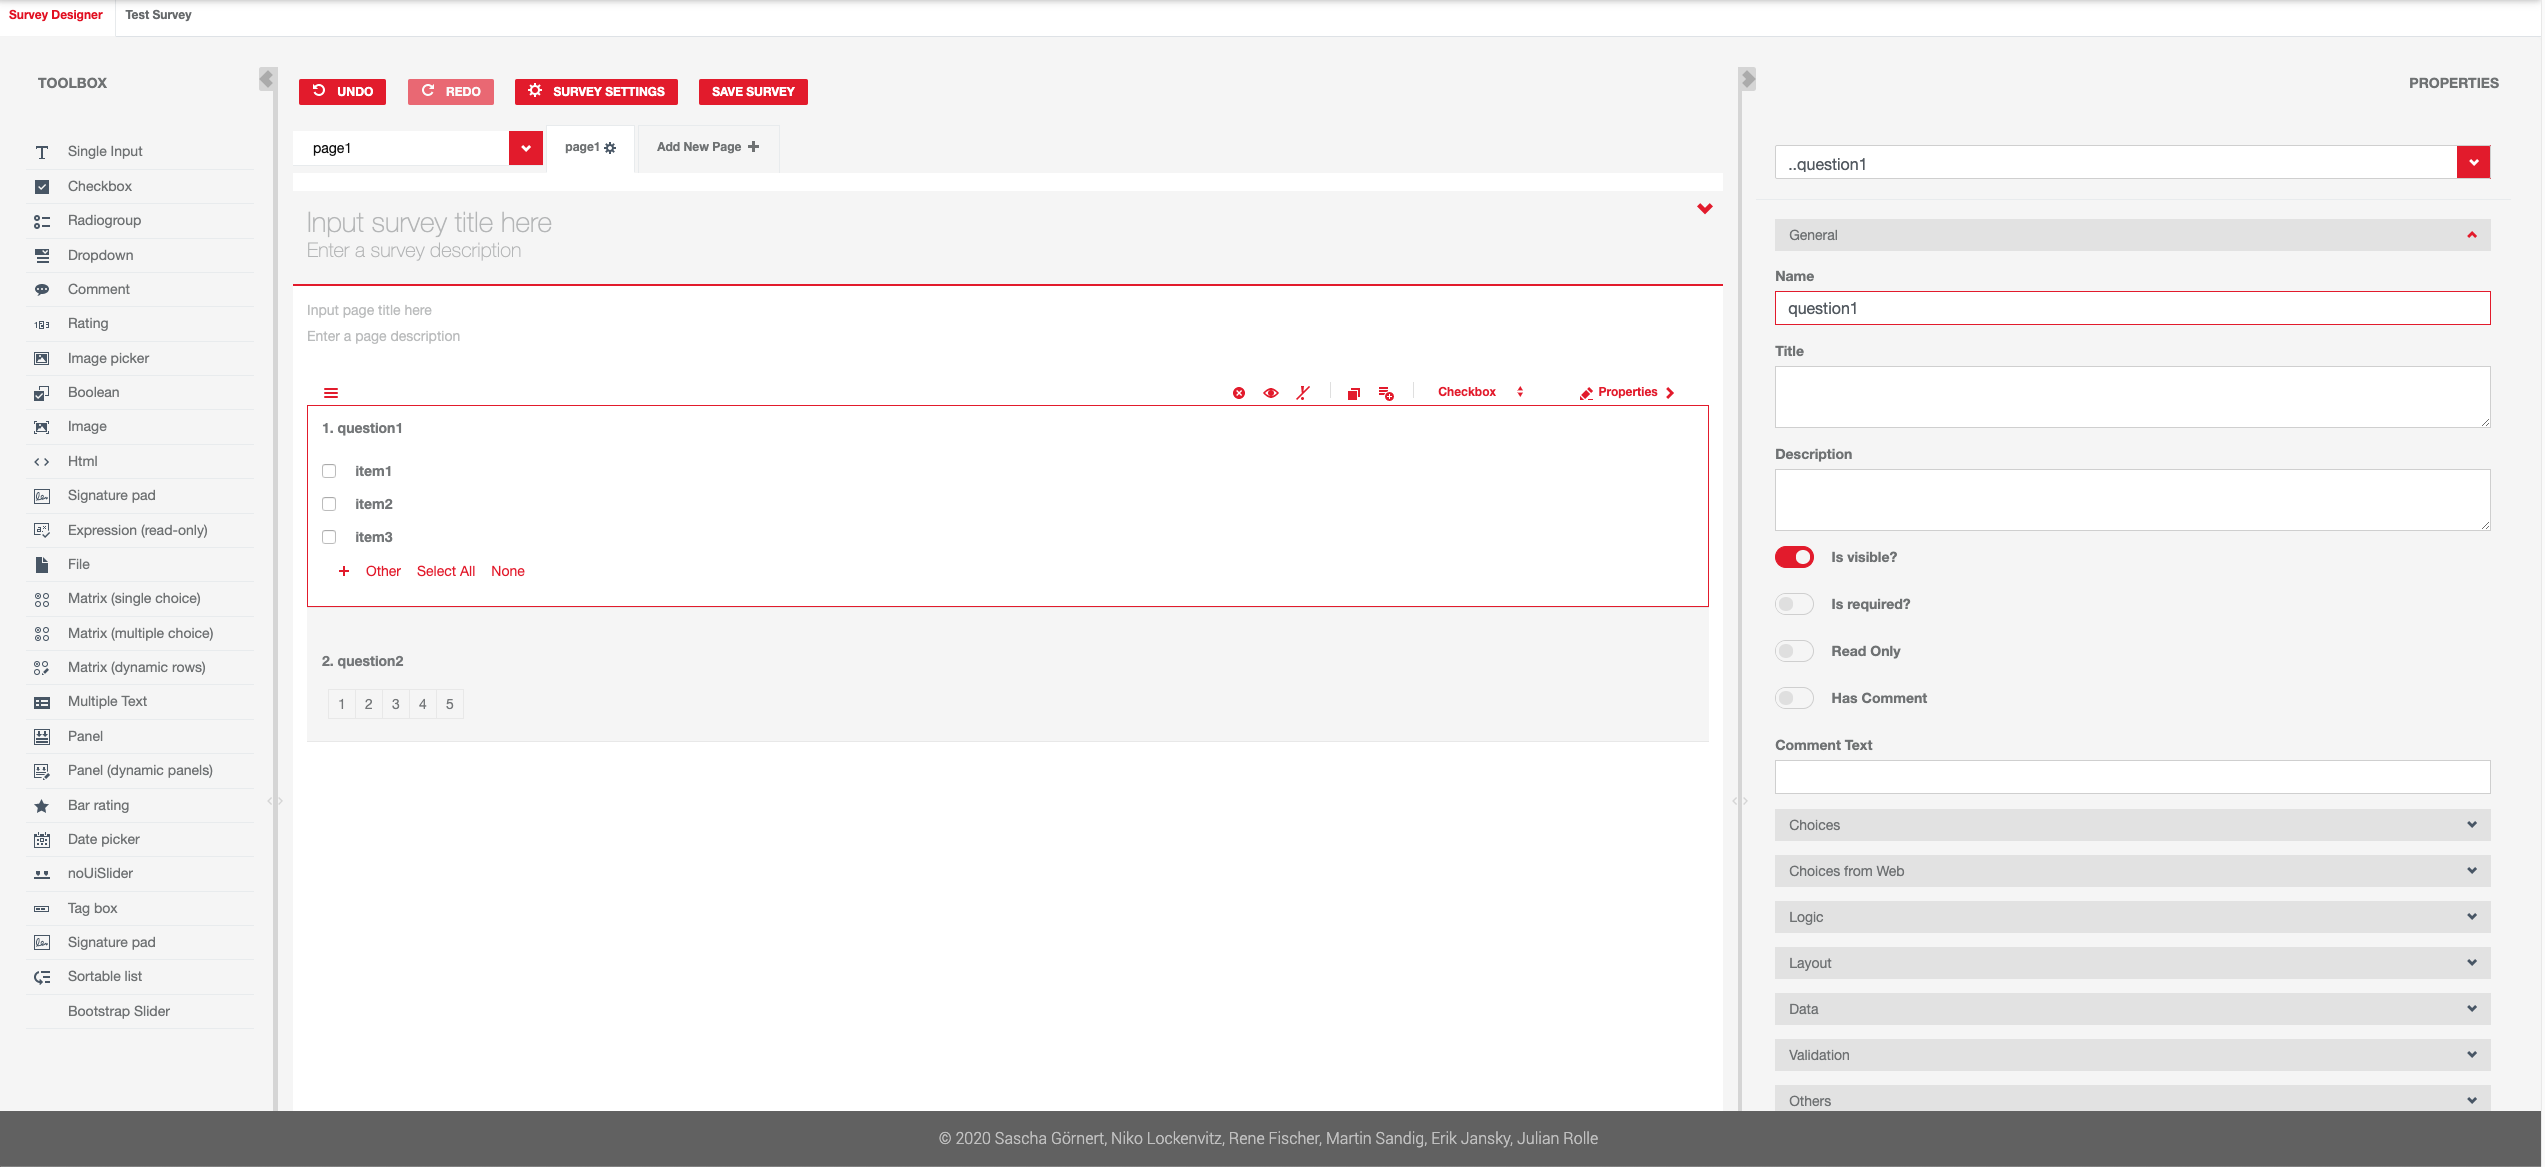
\includegraphics[width=0.95\textwidth, keepaspectratio]{img/client/CreateSurveyMaster.png}
	\captionsetup{justification=centering, format=plain}
	\caption[\acl{UI}: Erstellen einer Umfrage]{\acl{UI}: Erstellen einer Umfrage \\ \quelleScreenshot}
	\label{fig:SurveyCreatorImplement}
\end{figure}

Klickt der Benutzer auf die Schaltfläche \jinline|Test Survey|, werden die erstellten Umfragen dargestellt.
Dabei kann der Nutzer sehen, wie sich die Umfrage auf verschiedene Geräte, wie \zb einem iPhone 8, verhält.
Abbildung~\vref{fig:SurveyAnsicht} zeigt die Möglichkeit, die erstellte Umfrage auf einem bestimmten Gerät \engl{device} zu sehen (hier: Desktop).
Der Benutzer kann die Umfrage über eine Vorschau \engl{preview}, wie in Abbildung~\vref{fig:SurveyMobileAnsicht} dargestellt, auf verschiedenen mobilen Geräten betrachten.
Abbildung~\vref{fig:SurveyMobileAnsichtIPhone8} zeigt die erstellte Umfrage auf einem iPhone 8 an, wohingegen Abbildung~\vref{fig:SurveyMobileAnsichtAndroid} die Umfrage auf einem Android-Smartphone widerspiegelt.

\begin{figure}[!htb]
	\centering
	\captionsetup{justification=centering, format=plain}
	\subfigure[Ansicht der Umfrage]{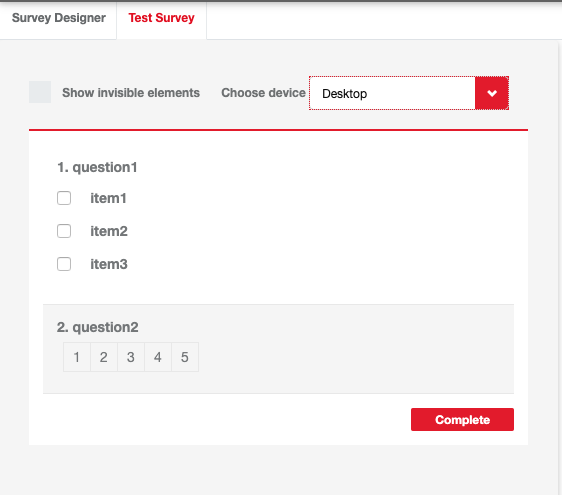
\includegraphics[width=0.48\textwidth]{img/client/CreateSurveyMaster_View1.png}\label{fig:SurveyAnsicht}}\hfill
	\subfigure[Auswahl verschiedener mobiler Ansichten]{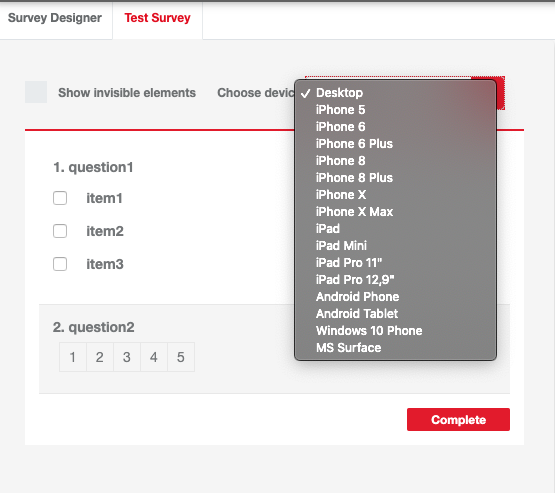
\includegraphics[width=0.48\textwidth]{img/client/CreateSurveyMaster_View2.png}\label{fig:SurveyMobileAnsicht}}\hfill
	\subfigure[Mobile Ansicht: iPhone 8]{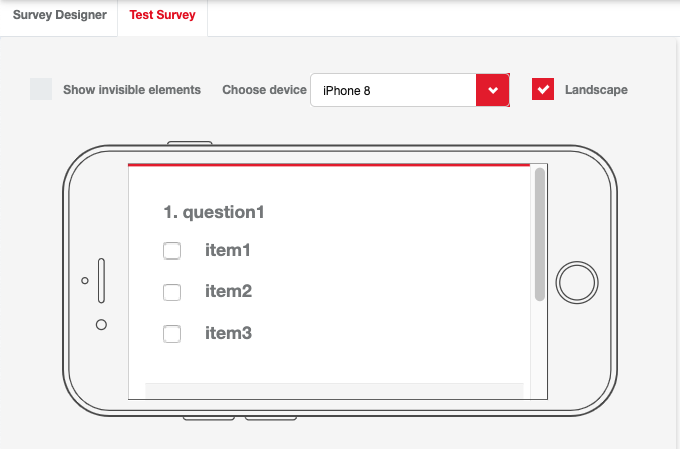
\includegraphics[width=0.48\textwidth]{img/client/CreateSurveyMaster_View3.png}\label{fig:SurveyMobileAnsichtIPhone8}}\hfill
	\subfigure[Mobile Ansicht: Android-Smartphone]{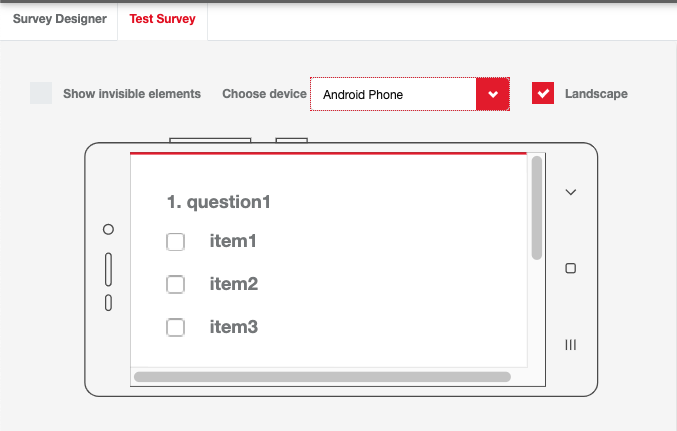
\includegraphics[width=0.48\textwidth]{img/client/CreateSurveyMaster_View4.png}\label{fig:SurveyMobileAnsichtAndroid}}
	\caption[\acl{UI}: Darstellung der erstellten Umfrage auf verschiedenen Geräten]{\label{fig:SurveyCreatorViewImplement}\acl{UI}: Darstellung der erstellten Umfrage auf verschiedenen Geräten \\ \quelleScreenshot}
\end{figure}

Über einen Knopf \jinline|Save Survey| kann der Benutzer die Umfrage speichern.
Zudem erhält der Nutzer ein visuelles Feedback über den Erfolg oder Nichterfolg des Erstellens der Umfrage.
Die erstellten Umfragen erscheinen im \emph{Survey Dashboard} (Kapitel~\vref{ssec:UmfrageDashboard}).
